\section{Evaluation}\label{sec:evaluation}

\subsection{Experimental Results}
Based on the MATLAB implementation, the data sets are processed and the networked SEIR model approach is applied. The results are evaluated from two different perspectives: 1) presentation and interpretation of results (numerically and graphically) for identification and simulation of a networked SEIR model for the complete time period, using combined mobility behavior and comparing the results with and without the use of the transient adjacency matrix and 2) comparison to the original results from \cite{vrabacCapturingEffectsTransportation2020}.

\subsubsection{Networked SEIR model identification and simulation results}
The networked SEIR model using German public transport data and mobility behavior data proves to be a very effective approach to model the COVID-19 outbreak even for the multiple waves that occurred until the time of writing. \autoref{fig:compAggrCombWave0} shows a comparison of the results for the networked SEIR model with and without use of the transient adjacency matrix $A3$ as introduced in \autoref{ssec:transientAdjancencyMatrixCalculation}. The plots show the denormalized data per compartment aggregated over the entire nation. As can be seen, the use of the transient adjacency matrix (subplots \autoref{fig:compAggrCombWave0Exp}, \autoref{fig:compAggrCombWave0Inf} and \autoref{fig:compAggrCombWave0Rem}) drastically improves simulation performance and successfully recovers the second and third outbreak.

To yield these results, the settings according to \autoref{tbl:seirSettings} were applied. The identified parameters and error figures are compared in \autoref{tbl:seirParametersAndError}.

As \autoref{tbl:seirParametersAndError} indicates, including the $A3$ adjacency matrix results in higher error of the normalized compartment, but reduces the error on denormalized levels per compartment. This relates well to the orange curves for the simulated pandemic levels in \autoref{fig:compAggrCombWave0}. The deviation on the normalized data presumably results from the incomplete model of the pandemic based on the mobility data alone, as other factors like policy, weather, virus variants, population structure are neglected in this analysis.

 The deviations of the model from the real outbreak data starting in April 2021 are likely attributable to the onset of vaccinations, which are not accounted for in the SEIR model and reduce the susceptible compartment, therefore reducing the pandemic activity.

Additionally, \autoref{fig:compAggrCombWave0} presents the possibility to simulate counterfactuals and check their impact with the identified model. As the plots suggest, the seemingly simple policy of limiting the railway usage to 50\% of 2019 levels might have reduced the pandemic activity by a large margin\footnote{Final levels of removed compartment: real: $3.7182{\times} 10^6$, simulated: $3.0049{\times} 10^6$, counterfactual: $1.8377{\times} 10^6$}.

\begin{table}[h]
     \centering
     \caption{Settings for the identification and simulation for 01-Feb-2020 to 23-Jun-2021}
     \begin{tabular*}{.75\linewidth}{l||l}
     Option & Value \\
     \hline
     \hline
     tLagRemoved & 7\\
     tLagDeath & 7\\
     tLeadExposed & 7\footnotemark\\
     tSmoothCases & 7\\
     h & 1\\
     mobilityLevel & combined\\
     counterfactual type & cappedTop\\
     counterfactual value & 0.5\\
     \hline
     \end{tabular*}
     \label{tbl:seirSettings}
\end{table}
\footnotetext{The RKI notes a median of 5-6 days and a 95th percentile of 10-14 days incubation period based on a survey of studies. \cite{robertkoch-institutrkiEpidemiologischerSteckbriefSARSCoV22021}}

\begin{table}[h]
     \centering
     \caption[]{Identification results and error metrics\footnotemark of the networked SEIR model for 01-Feb-2020 to 23-Jun-2021}
     \begin{tabular*}{\linewidth}{l||p{3.1cm}|p{3.1cm}}
     Metric & $A3 \neq 0$ & $A3 = 0$ \\
     \hline
     \hline
     $\beta_E$ &$[6.8 {\times} 10^{\shortminus5},\linebreak[1] 0.1354,$\newline$ 0.0574]$ &$[6.3 {\times} 10^{\shortminus8},\linebreak[1] 0.1497,$\newline$ 0]$\\
     $\beta_I$ &$[1.8 {\times} 10^{\shortminus5},\linebreak[1] 7.8 {\times} 10^{\shortminus7},\linebreak[1] 3.3 {\times} 10^{\shortminus4}]$ &$[9 {\times} 10^{-9},\linebreak[1] 2.8 {\times} 10^{\shortminus8},\linebreak[1] 0]$\\
     $\sigma$ &$0.1395$ &$0.1390$\\
     $\gamma$ &$0.1394$ &$0.1392$\\
     $\frac{\lVert e_{real} - e_{sim} \rVert}{\lVert e_{real} \rVert}$ &$1.955, 0.4588$ &$1.132, 0.9379$\\
     $\frac{\lVert i_{real} - i_{sim} \rVert}{\lVert i_{real} \rVert}$ &$2.023, 0.4641$ &$1.130, 0.9379$\\
     $\frac{\lVert r_{real} - r_{sim} \rVert}{\lVert r_{real} \rVert}$ &$2.039, 0.4588$ &$1.076, 0.9457$\\
     \hline
     \end{tabular*}
     \label{tbl:seirParametersAndError}
\end{table}
\footnotetext{Two error metrics are presented per compartment. The first one is calculated on normalized compartment levels, while the second one is calculated on aggregated, denormalized levels.}
    
\begin{figure}[hbtp]
     \centering
     \begin{subfigure}[b]{.45\linewidth}
         \centering
         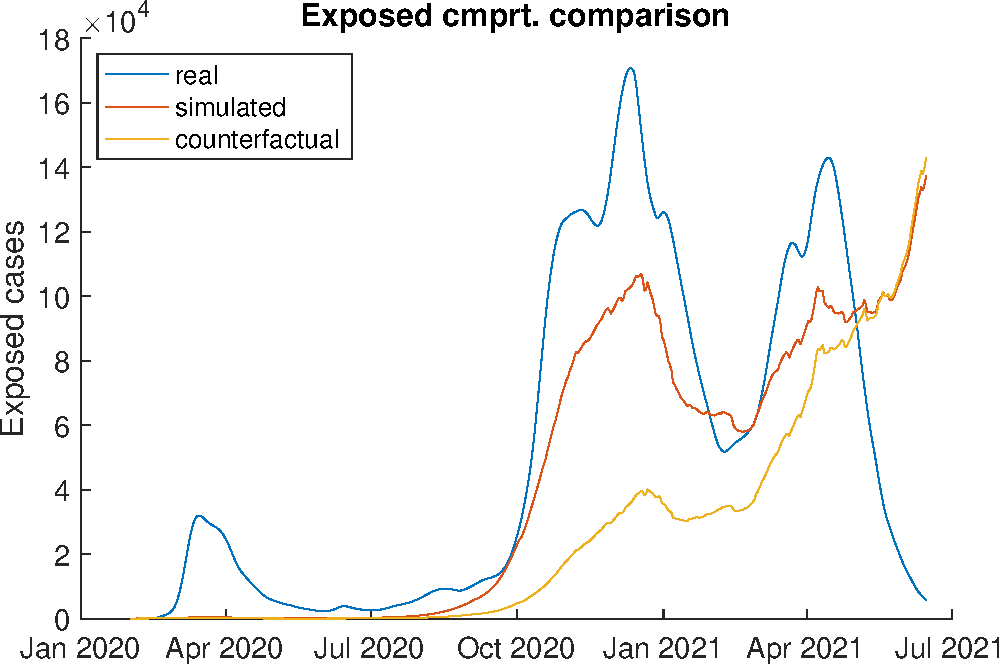
\includegraphics[width=\linewidth]{img/210907_171119_combined_wave0/figures/COMP_exp}
         \caption{Exposed, $A3 \neq 0$}
         \label{fig:compAggrCombWave0Exp}
     \end{subfigure}
     \hfill
     \begin{subfigure}[b]{.45\linewidth}
         \centering
         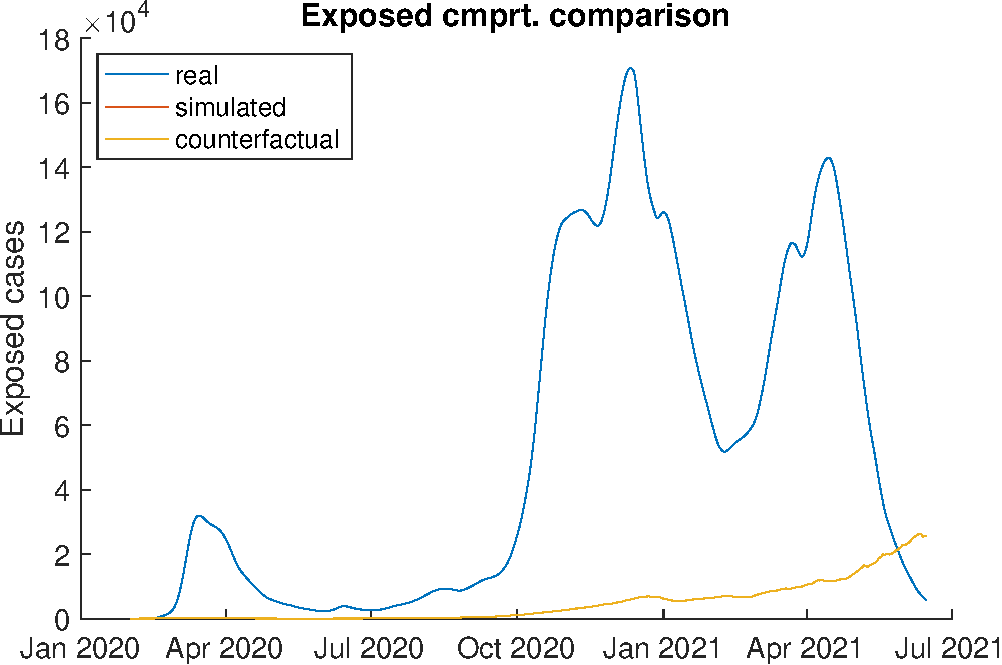
\includegraphics[width=\linewidth]{img/210907_180927_combined_wave0_noa3/figures/COMP_exp}
         \caption{Exposed, $A3 = 0$}
         \label{fig:compAggrCombWave0NoA3Exp}
     \end{subfigure}
     \newline
     \begin{subfigure}[b]{.45\linewidth}
         \centering
         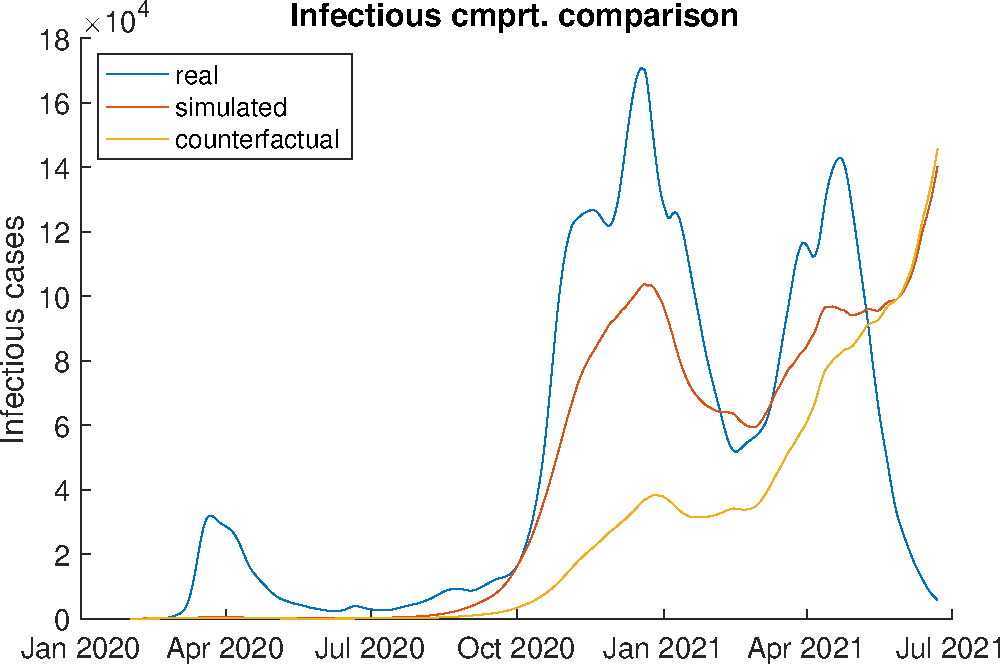
\includegraphics[width=\linewidth]{img/210907_171119_combined_wave0/figures/COMP_inf}
         \caption{Infectious, $A3 \neq 0$}
         \label{fig:compAggrCombWave0Inf}
     \end{subfigure}
     \hfill
     \begin{subfigure}[b]{.45\linewidth}
         \centering
         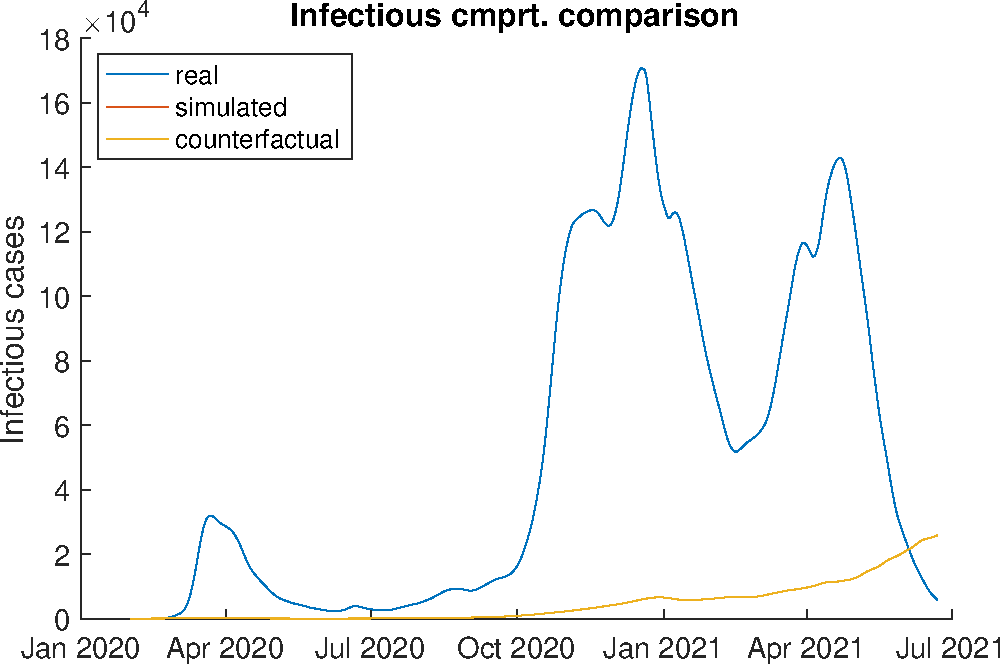
\includegraphics[width=\linewidth]{img/210907_180927_combined_wave0_noa3/figures/COMP_inf}
         \caption{Infectious, $A3 = 0$}
         \label{fig:compAggrCombWave0NoA3Inf}
     \end{subfigure}
     \newline
     \begin{subfigure}[b]{.45\linewidth}
         \centering
         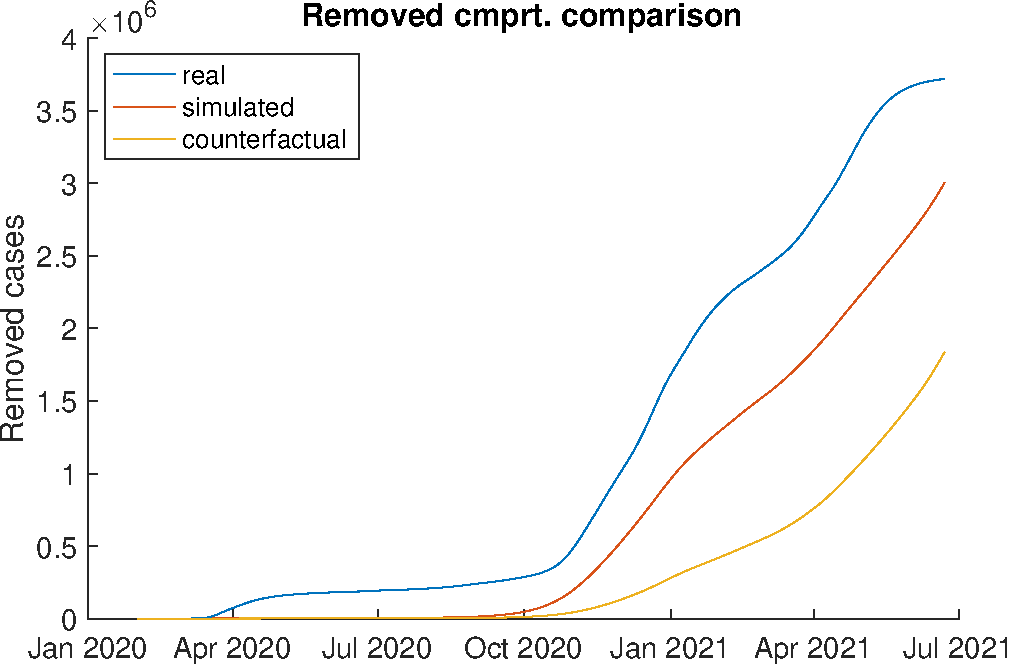
\includegraphics[width=\linewidth]{img/210907_171119_combined_wave0/figures/COMP_rem}
         \caption{Removed, $A3 \neq 0$}
         \label{fig:compAggrCombWave0Rem}
     \end{subfigure}
     \hfill
     \begin{subfigure}[b]{.45\linewidth}
         \centering
         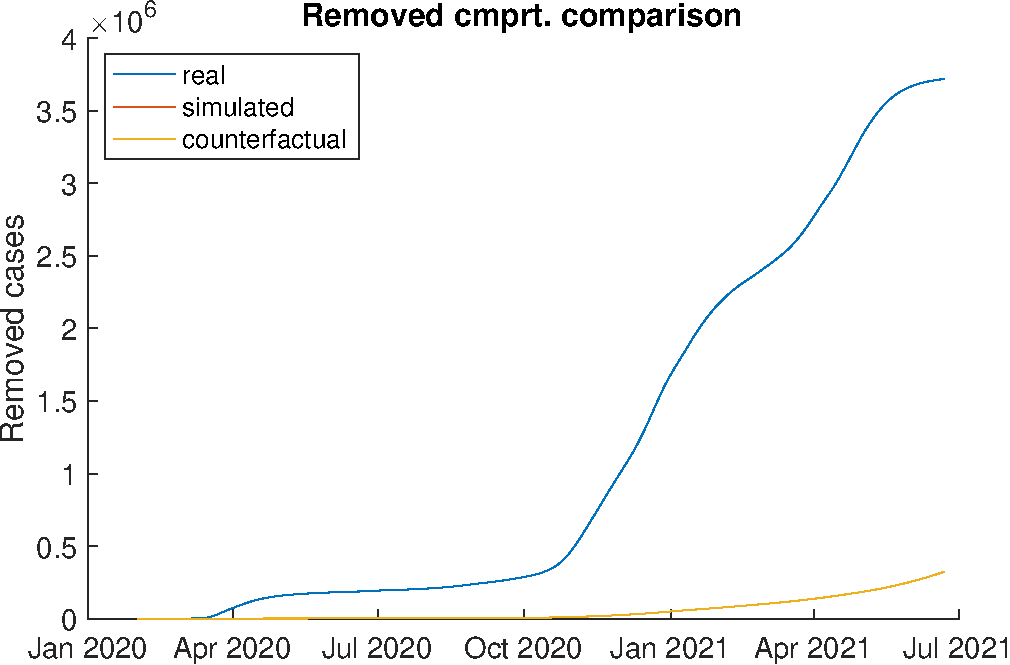
\includegraphics[width=\linewidth]{img/210907_180927_combined_wave0_noa3/figures/COMP_rem}
         \caption{Removed, $A3 = 0$}
         \label{fig:compAggrCombWave0NoA3Rem}
     \end{subfigure}     
     \caption[Comparison of aggregated, denormalized compartment levels of networked SEIR model with and without $A3$]{Comparison of aggregated, denormalized compartment levels of networked SEIR model with and without $A3$\protect\footnotemark}
     \label{fig:compAggrCombWave0}
\end{figure}
\footnotetext{The counterfactual line represents the outcome of a theoretical change in the usage behavior of public transport. The plots show the results of applying upper bounded ($50 \%$) behavior data as $\psi_{3_j}$. The simulated and counterfactual lines intersect for subplots (b), (d) and (f) as $A3=0$.}

\subsubsection{Comparison to the results of Vrabac et al.}
This work differs to the approach and results presented in \cite{vrabacCapturingEffectsTransportation2020} in the following categories:

\begin{itemize}
	\item The scope of analysis is the entire set of counties of Germany instead of a subset of counties from the U.S.
	\item The time range includes not just the first COVID-19 outbreak but considers all three waves that occurred until the time of writing.
	\item The scaling of the adjacency matrix is performed based on measured mobility behavior--which correlates with policy information--instead of guessed parameters.
	\item The analysis is validated against denormalized data.
\end{itemize}
